%%%%%%%%%%%%%%%%%%%%%%%%%%%%%%%%%%%%%%%%%%%%%%%%%%%%%%%%%%%%%%%%%%%%%%%%%%%%%%%%%%%%%%%%%%%%%%%%%%%%%%%
% Sablona pro projekty ekonometrickych predmetu                                                     %%%
% Vytvoreno v ramci grantu: Ekonometricke nastroje a techniky v realnych ekonomickych aplikacich    %%%
% Autor: Jakub Bucek (jakubbucek@mail.muni.cz)                                                      %%%
% Pripominky, dotazy, namety smerujte na autora nebo na Daniela Nemce (danek@mail.muni.cz)		    %%%
% Vytvoreno: 1.12.2014                                                                              %%%
%%%%%%%%%%%%%%%%%%%%%%%%%%%%%%%%%%%%%%%%%%%%%%%%%%%%%%%%%%%%%%%%%%%%%%%%%%%%%%%%%%%%%%%%%%%%%%%%%%%%%%%

\documentclass[12pt,a4paper,oneside,final]{article}

%%%%%%%%%%%%%%%%%%%%%%%%%%%%%%%%%%%%%%%%%%%%%%%%%%%%%%%%%%%%%%%%%%%%%%%%%%%%%%%%%%%%%%%%%%%%%%%%%%%%%%%
%%%%%%%%%%%%%%%%%%%%%%%%%%%%%%%%%%%%%% ZAKLADNI NASTAVENI %%%%%%%%%%%%%%%%%%%%%%%%%%%%%%%%%%%%%%%%%%%%%

%% Nastaveni kodovani
\usepackage[utf8]{inputenc} 
\usepackage[IL2]{fontenc} %% fonty vhodne pro sazbu ceskych a slovenskych dokumentu
\usepackage[slovak]{babel}

%% Fonty
\usepackage{mathptmx}  %% volne dostupny font Adobe Times Roman
% \usepackage{bookman}
% \usepackage{charter}
% \usepackage{fourier}
% \usepackage{mathpazo}
% \usepackage{newcent}
% \usepackage{palatino}
% \usepackage{utopia}

%% Baliky potrebne pro sazbu matematiky
\usepackage{amssymb,amsthm,amsmath}
\usepackage{bm}
\usepackage{tabularx} %% vylepsene tabulky

%% Balik nutny pro sablonu
\usepackage{garfield} %% nacteni stylu sablony

%% Vlastní definice
\renewcommand\vec[1]{\ensuremath\boldsymbol{#1}} %% tucne vektory
\newtheorem{veta}{Věta}[section]
\swapnumbers
\theoremstyle{definition}
\newtheorem{definice}{Definice}
\theoremstyle{remark}
\newtheorem*{pozn}{Poznámka}
\numberwithin{equation}{section}

%%%%%%%%%%%%%%%%%%%%%%%%%%%%%%%%%%%%%%%%%%%%%%%%%%%%%%%%%%%%%%%%%%%%%%%%%%%%%%%%%%%%%%%%%%%%%%%%%%%%%%%
%%%%%%%%%%%%%%%%%%%%%%%%%%%%%%%%%%%%%%%% TITULNI STRANA %%%%%%%%%%%%%%%%%%%%%%%%%%%%%%%%%%%%%%%%%%%%%%%

\NazevPrace{Predikcia časových radov}
\Autor{BC. Pavol Loffay}
\Univerzita{Masarykova univerzita}
\Fakulta{Fakulta informatiky}
\Obor{Service Science Management Engineering}
\Mail{p.loffay@mail.muni.cz}
\DatumOdevzdani{\today}
\Abstrakt{
 Práca spracováva predikciu časových radov prevziatych z monitorovacieho sýstému
 Hawkular\footnote{Dostupné na http://www.hawkular.org}. Tento systém dokáže
 monitorovať Java aplikácie, alebo fyzický stroj na ktom je spustený.
 Z množiny pozorovaných metrík som vybral následujúce: vyťaženie Java hromady (heap),
 miesto na disku a počet voľných databázových spojení. Tieto časové rady som analyzoval
 a cieľom bolo zostaviť model, ktorý nejlepšie popisoval priebeh danej časovej rady. 
 V práci som postupoval podľa Box\,--\,Jenkinsových motód.
}
\KlicovaSlova{Časová rada; ARIMA; Hawkular; ACF}
\JELklasifikace{C53}

%%%%%%%%%%%%%%%%%%%%%%%%%%%%%%%%%%%%%%%%%%%%%%%%%%%%%%%%%%%%%%%%%%%%%%%%%%%%%%%%%%%%%%%%%%%%%%%%%%%%%%%
%%%%%%%%%%%%%%%%%%%%%%%%%%%%%%%%%%%%%% ZACATEK DOKUMENTU %%%%%%%%%%%%%%%%%%%%%%%%%%%%%%%%%%%%%%%%%%%%%%

\begin{document}
\VytvorTitulniStranu

\section{Úvod}
\cite{cipra} \cite{brockwell_ts}Povšimněte si prvního odstavce, který není podle~standardních pravidel \LaTeX{u} odsazen. Všechny ostatní odstavce již odsazeny jsou; jsou formátovány automaticky, proto jen vždy začněte nový odstavec buď odřádkováním, nebo příkazem \verb|\par|. Mezi~odstavci je nastavené automatické řádkování 6 bodů, proto prosím nepoužívejte žádné další příkazy na řádkování. Všimněte si ještě tohoto \emph{zvýrazněného} slova a také tohoto \textbf{velmi důležitého} slova (ke~zvýraznění použijte příslušné styly).

Většina článků začíná stručným představením toho, jaké otázky jsou řešeny, co vás k~jejich řešení vedlo a shrnuje dosažená empirická zjištění. Úvod by  měl být většinou psán jednoduchým \uv{netechnickým} jazykem s~minimem odborných ekonomických a statistických výrazů. I laický čtenář by tak měl obecně pochopit problém a získané závěry, které jsou v~projektu či příspěvku řešeny. Právě na~tomto místě je nejlepší příležitost k~tomu, vyzdvihnout originalitu a přínos vašeho článku, tedy čím je zajímavý a proč má cenu ho vůbec číst. Není od~věci přehledně představit i obsah jednotlivých částí zprávy.

Na~úvod ještě uveďme, že zde navrhované názvy nejsou nijak závazné a můžete jednotlivé kapitoly nazvat i jinými, originálnějšími názvy, které lépe vystihují daný problém. 

\section{Ekonomický model}

Tato část obsahuje formální popis teoretického modelu. Obvykle je techničtěji založená a využívá se zde více jazyk ekonomie a matematiky. V~této části je možné se zaměřit na~posluchače, kteří jsou experty v~daném oboru. V~této části je věnován prostor specifikaci používaného ekonomického modelu a definování ekonomických proměnných.

Ekonomický model může být mnohdy rozsáhlý a komplikovaný. Vaším úkolem je vysvětlit model zcela jasně, a to co nejstručněji a nejjednodušším způsobem. Není třeba používat ryze technického žargonu. Kde je to možné, snažte se používat jednoduchých a výstižných pojmů a obratů namísto zbytečně komplikovaných výrazů. Vašim cílem je ukázat kvalitu vašich myšlenek, nikoli šíří a rozsah vaši slovní zásoby.

Vhodnou součástí vaší práce je seznámení čtenářů s~aktuální úrovní výzkumu daného tématu. Není ovšem nutné představovat přehled veškeré literatury, která se k~danému tématu vztahuje. Na~odbornou literaturu se můžete odkazovat pomocí příkazu \verb|\cite{label}|, například \uv{Enders \cite{enders2010} uvádí $\dots$} nebo \uv{Podle~\cite{enders2010} můžeme $\dots$}. Zkuste si odpovědět na~otázky: Věnoval se tomuto konkrétnímu tématu již někdo před~vámi? Pokud ano, jaké jsou závěry jeho práce? Bude vaše práce něčím daný problém rozšiřovat nebo jenom replikujete dané metody pro~jiná data?

Na~závěr této sekce byste si měli stanovit jednu až dvě pracovní hypotézy, které budete v~práci testovat a které by měly být nejdůležitějším prvkem vaší práce. Nesnažte se stanovovat moc obecné hypotézy (např. jestli globalizace má vliv na~ekonomický růst\footnote{Takové obecné hypotézy stejně potřebují konkretizovat ve~smyslu, co je myšleno globalizací a co ekonomickým růstem.}) nebo naopak takové hypotézy, u~kterých je na~první pohled patrné, že platí/neplatí (např. velká auta mají větší spotřebu jako malá auta). Příkladem vhodné hypotézy v~případě, že se vaše práce bude věnovat problému spropitného, je například, jestli muži dávají v~průměru vyšší spropitné než ženy a jaké je případná velikost tohoto rozdílu.

\section{Ekonometrický model}

V~této části byste měli čtenáři představit ekonometrické nástroje, které využijete při~své analýze. Není nutné uvádět ty techniky, které jsou známy průměrnému vzdělanému člověku daného oboru. V~případě předmětu \emph{Základy ekonometrie} tedy není nutné vysvětlovat čtenáři, co je to lineární regrese a že se její koeficienty odhadují pomocí metody nejmenších čtverců. Uvádějte jen ty metody, které nejsou v~daném oboru běžné. 

Jelikož se předpokládá, že v~této sekci naplno využijete sazby matematiky, kterou nabízí \LaTeX{}, obsahuje tento balíček tyto předdefinované prostředí a funkce. Pomocí příkazů \verb|\Cbb, \Rbb, \Zbb, \Nbb| můžete vysázet tučné symboly pro~číselné obory $\Cbb, \Rbb, \Zbb, \Nbb$.

Dále pomocí příkazu \verb|\e{x}| lze vysázet $\e{x}$ (všimněte si rozdílu mezi $e^x$ a $\e{x}$), lze použít i \LaTeX{ový} příkaz \verb|\exp{x}|, jež po~vysazení vypadá takto $\exp{x}$. Především při~sazbě integrálu můžete použít příkaz \verb|\dif{x}| -- viz rozdíl $\int f(x) dx$ a $\int f(x) \dif{x}$. 

Při~maximalizačních či minimalizačních úlohách můžete využít předdefinovaných operátorů \verb|\argmax| nebo \verb|\argmin|, které lze kombinovat např. i s~předchozími příkazy, viz vzorec \ref{vzorec}. Dalším předdefinovaným operátorem je \verb|\sqn|, který vysází operátor signum $\sgn$.

\begin{equation}
\beta = \argmax_{x \in \Rbb} \int_0^x \sin{t} \e{-t} \dif{t}
\label{vzorec}
\end{equation}

Tato šablona obsahuje také podporu základním statistickým funkcím. Najdete zde příkaz \verb|\E{X}|, který sází střední hodnotu $\E{X}$. Dále příkaz \verb|\Var{X}| na~vysázení rozptylu $\Var{X}$, příkaz \verb|\Cov{X}{Y}| na~vysázení kovariance $\Cov{X}{Y}$ a příkaz \verb|\Cor{X}{Y}| na~vysázení $\Cor{X}{Y}$.

Příkaz \verb|\vec{}| je modifikovaný tak, aby místo šipky nad~svým argumentem, tento argument vysázel tučně, např. tučné $\vec{\alpha}, \vec{\beta}, \vec{\gamma}$ oproti normálnímu $\alpha, \beta, \gamma$.

Pro~opravdové matematické \uv{fajnšmekry} jsou v~šabloně nachystány i prostředí \verb|veta|, \verb|definice| a \verb|pozn|. Lze použít i \LaTeX{ovské} prostředí \verb|proof|.

\begin{veta}[Moje]
Moje věta.
\end{veta}

\begin{proof}
Zde je důkaz předchozí věty, jehož konec poznám pomocí čtverečku napravo.
\end{proof}

\begin{definice}
Moje definice.
\end{definice}

\begin{pozn}
Moje poznámka.
\end{pozn}

\section{Data}

Touto částí začíná část s~empirickými výsledky vaší práce. Měla tvořit hlavní a nejdůležitější část vaší práce. Rozsahem by měla odpovídat přibližně polovině rozsahu celé práce. V~této části byste měli nejprve představit data, se~kterými pracujete. Někdy se v~této části zmiňuje i program, popř. jeho balíčky, ve~kterém jste data zpracovávali. Dále byste měli uvést odhady modelu, případně zkontrolovat i splnění jeho předpokladů. Jako poslední přichází na~řadu interpretace výsledků, což je nejzásadnější část celé práce, proto byste ji měli věnovat zvýšenou pozornost. Zkuste si odpovědět na otázky: Jsou odhadnuté koeficienty významné nebo jsou p-hodnoty jen těsně nad~zvolenou hladinou významnosti (při~menším počtu pozorování je vhodné pracovat s~větší hladinou významnosti)? Jsou výsledky v~souladu s~vaší představou? Je model správně specifikovaný? Zvolili jste správný datový vzorek? Zamítáte či nezamítáte hypotézy stanovené na~začátku práce?

Jelikož pracujete s~reálnými daty\footnote{Doporučujeme si přečíst přílohu D učebního textu, ve~kterém se blíže seznámíte, jak pracovat s~datovými databázemi.}, je potřeba s~nimi čtenáře seznámit. Měli byste začít s~tím, že uvedete zdroj, odkud vaše data pocházejí. Pokud data pocházejí z~dotazníkového šetření, můžete uvést podobu dotazníku v~příloze~\ref{priloha} společně s~popisem cílové skupiny, která na~tento dotazník odpovídala. V~případě, že jste museli nějakým způsobem vaše data transformovat, nezapomeňte tuto skutečnost do~práce také napsat.

Pro~vyšší názornost je vhodné data vizualizovat, viz Obrázek~\ref{obr:example}.

% priklad obrazku
\begin{figure}[htb]
\centering
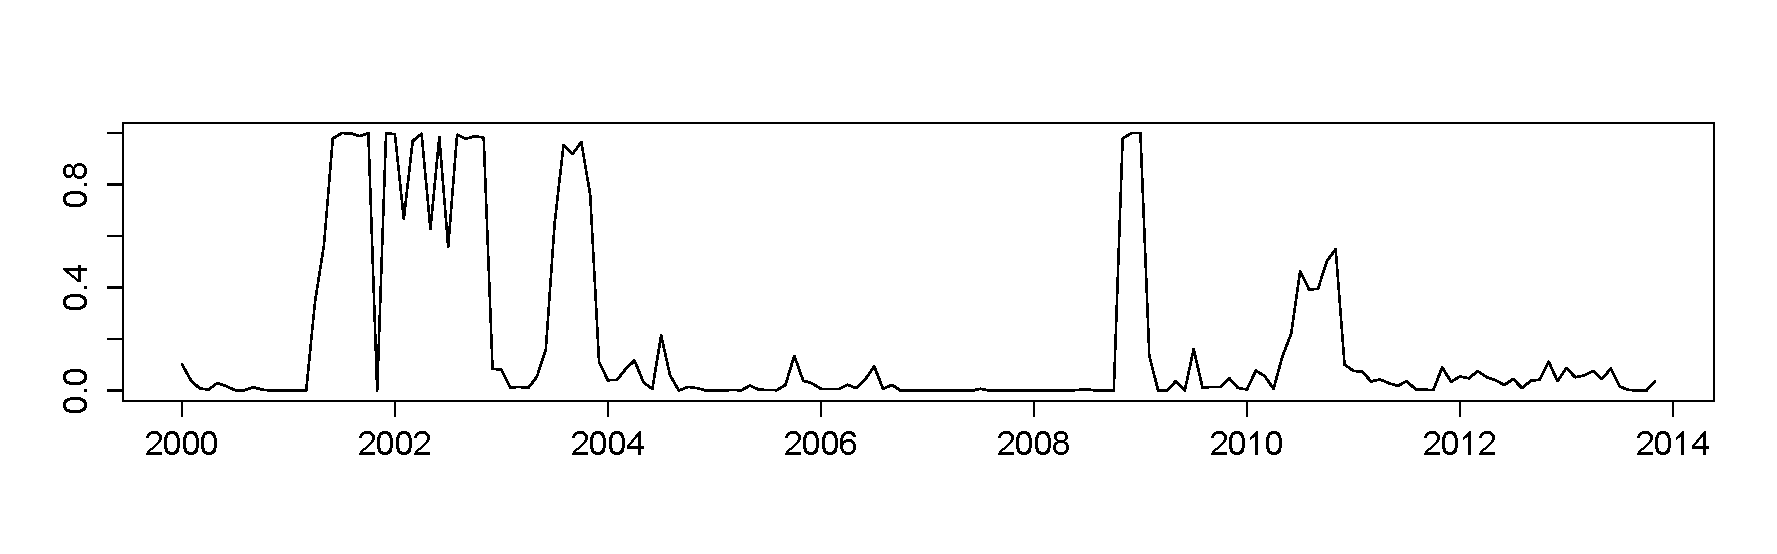
\includegraphics[width=.9\textwidth]{images/example.pdf}
\caption{Pod~obrázkem by měl následovat popis grafu společně s~uvedením \textbf{zdroje}.}
\label{obr:example} % unikatni navesti, pomoci ktereho se budeme v textu odvolavat na dany obrazek
\end{figure}

Standardně se v~podobných článcích vyskytuje i tabulka se~základními popisnými charakteristikami, viz Tabulka~\ref{tab:charakteristiky}\footnote{Tabulky uvedené v~této šabloně jsou pouze příklady, jak může formátování tabulek vypadat a nemusíte se tohoto formátování striktně držet. Může volit vlastní formát, kde se preferuje co nejjednodušší použití čar (pro~přehlednost tabulek).}.

% priklad tabulky
\begin{table}[htb]
\caption{Pod~tabulkou by měl následovat popis tabulky společně s~uvedením \textbf{zdroje}.}
\centering
\begin{tabular}{cccccc}
\textbf{Proměnná} & \textbf{Průměr} & \textbf{Sm. odchylka} & \textbf{Minimum} & \textbf{Maximum} \\
\hline
Proměnná1 & 10 & 1,2 & 7 & 12  \\
Proměnná2 & 5 & 1 & 3 & 4,7  \\
$\vdots$ & $\vdots$ & $\vdots$ & $\vdots$ & $\vdots$ \\
\hline
\end{tabular}
\label{tab:charakteristiky}
\end{table}

\section{Odhadnutý model}

Všechny statistické metody, které využíváte, jsou zkonstruované na~základě jistých předpokladů. Zde přichází vhodné místo, kdy je potřeba splnění těchto předpokladů testovat. Testování některých předpokladů můžete rozdělit do~dalších podsekcí (pomocí příkazu \verb|\subsection{}| pro~číslovanou variantu a \verb|\subsection*{}| pro~nečíslovanou variantu), např. pro~ilustraci: Odhad lineární specifikace a Odhad log-lineární specifikace.

Pro~vysázení těchto předpokladů můžete využít například i seznamy.

\begin{minipage}[c]{.45\textwidth}
Nečíslovaný seznam:
\begin{itemize}
\item jedna
\item dva
\item tři
\end{itemize}
\end{minipage} %
\begin{minipage}[c]{.45\textwidth}
Číslovaný seznam:
\begin{enumerate}
\item jedna
\item dva
\item tři
\end{enumerate}
\end{minipage}

Dále byste měli v~této části přepsat do~přehledné tabulky odhady koeficientů společně s~jejími směrodatnými hodnotami a jejich významností, viz Tabulka~\ref{tab:koef}. Nedoporučuje se kopírovat výsledky v~podobě \uv{screenshotu}, který poté vložíte jako obrázek do~textu. Program \emph{Gretl} nabízí jako jeden z~výstupu \LaTeX{}, který vám vygeneruje automaticky kód, který poté stačí jen zkopírovat do~šablony.

%% Pri sazbe cestiny muze mit Latex problemy se znakem "-".
%% Proto obalte dane misto, kde se "-" vyskytuje, dvojici prikazu "\shorthandoff{-}" a "\shorthandon{-}"
%% V tomto pripade by mel LaTeX problem s prikazem \cline

\shorthandoff{-}
\begin{table}
\centering
\caption{Pod~tabulkou by měl následovat popis tabulky společně s~uvedením \textbf{zdroje}.}
\begin{tabularx}{.75\textwidth}{lcc}
\textbf{Proměnná} & \textbf{Model A} & \textbf{Model B} \\
\hline
Proměnná1		& 10,56841 ***   & \\
 		   		& (2,54851)      & \\
Proměnná1Mod	&		   		 & 5,87787 *** \\
 				&		  		 & (1,00155) \\  
Proměnná2   	& 50,56984 ***   & 47,59663 *** \\
				& (5,00527)		 & (4,55953) \\
Proměnná3		& 20,96541 *     & 25,05194 ** \\
				& (3,64164)	   	 & (3,70647) \\
Proměnná4		& 17,87406       & 113,33046 * \\
				& (40,22301)     & (7,29106) \\
\hline
Koeficient determinace  & 0,822118		 & 0,842665 \\
F test                  & 21,78750 ***	 & 20,56845 *** \\
Durbin--Watson			& 0,007214 		 & 0,26546 \\
Test Jarque--Bery       & 10,3663 *** 	 & 9,59123 *** \\
\hline
\multicolumn{3}{X}{\footnotesize Pozn. v~závorkách jsou uvedeny směrodatné odchylky odhadu parametrů, které jsou odhadovány s~využitím robustních odhadů (Neweyho-Westův HAC estimátor);} \\
\multicolumn{3}{X}{\footnotesize *, **, *** označuje hladinu významnosti 10\,\%, 5\,\%, 1\,\%.}
\end{tabularx}
\label{tab:koef}
\end{table}
\shorthandon{-}

\section{Interpretace výsledků}

Jakmile máte odhadnutý model, který splňuje všechny předpoklady kladené na~tento model, měli byste být schopni vhodně interpretovat dosažené výsledky vzhledem ke~stanoveným pracovním hypotézám na~začátku práce.

Na~tomto místě je vhodné zdůraznit, že neexistují \uv{dobré} ani \uv{špatné} empirické výsledky. V~mnoha případech může nastat, že empirické výsledky nepotvrdí původní představu výzkumníka a ten může být zklamaný. V~ideálním světě přichází výzkumník s~novou teorií, provede empirickou práci a ta mu potvrdí jeho domněnku. Reálný svět je jiný. Proměnnou, která by měla být statisticky významná, identifikuje náš model jako statisticky nevýznamnou nebo koeficienty, které měly být kladné, mohou být někdy záporné. Je třeba mít na~paměti, že zjištění, že nějaká teorie nepopisuje realitu dostatečně přesně, je stejně hodnotné jako zjištění, že tato teorie funguje velice dobře. Nemusíme proto zoufat, když nějaké takové zdánlivě špatné výsledky dostaneme. Vždy si ovšem musíme zkontrolovat (i v~případě výsledků souhlasících s~nějakou teorií), že jsme postupovali korektním způsobem. Nejhorším přístupem je nějakým způsobem \uv{šolichat} s~daty či metodami, aby to \uv{vyšlo pěkně} (a navíc tyto pochybní metody zatajovat a tvářit se, že jsme postupovali korektně).   

Empirické výsledky mohou být někdy zavádějící. Jeden statistický test může identifikovat jednu věc, druhý naopak věc zcela opačnou. Vysvětlující proměnná, která je v~jednom modelu nevýznamná, může v~dalším modelu vyjít jako významná. V~takovém případě toho moc neuděláme a tyto výsledky ve~vší počestnosti zveřejníme (nevybereme si jen ten výsledek, který se nám hodí) a pokusíme se v~rámci možností porozumět tomu, proč takováto nejasnost vzniká a jaké může mít logické vysvětlení. 

\section{Záver}


\section*{Poďakovanie}

Na záver by som chcel poďakovať Ing. Danielovi Němcovi, Ph.D. za návrh na vypracovanie
tejto témi a za veľmi príjemné a užitočné konzultácie. Ďalej by som chcel poďakovať Ester
Železňákovej za gramatickú korektúru textu.

\bibliographystyle{czechiso}
\bibliography{bibliography}

%% Pokud nechcete pouzit prilohy, muzete nasledujici radky az po \end{document} smazat
\newpage
\renewcommand{\thesection}{\Alph{section}}
\setcounter{section}{0}
\renewcommand{\thepage}{\roman{page}}
\setcounter{page}{1}
\section{Přílohy}
\label{priloha}

Zde můžete uvést přílohy.

\end{document}

